\documentclass{article}
\setlength{\headheight}{25pt}
\usepackage{pgfplots}
\pgfplotsset{compat=1.16}
\usepackage{josuamathheader}
\begin{document}
    \section*{Aufgabe 1}
    Für die benötigte Energie gilt $Q = c \cdot m \cdot \Delta T$. Die durch das Schütteln aufgebrachte Wärmeenergie kann berechnet werden, indem einfach die gedachte Gesamthöhe, aus der das Wasser fällt durch Addieren der einzelnen Höhen berechnet wird: $Q = E_{\text{pot}} = m \cdot g \cdot h_\text{ges} = m \cdot g \cdot h \cdot \frac{1}{\mathrm{s}} \cdot t$. Gleichsetzen ergibt
    \begin{align*}
        c \cdot m \cdot \Delta T &= m \cdot g \cdot h \cdot \frac{1}{1\mathrm{s}} \cdot t\\
        t &= \frac{c \cdot \Delta T}{g \cdot h} \cdot 1\mathrm{s}\\
        &= \frac{4190 \cdot 85}{9.81 \cdot 0.3}\mathrm{s}\\
        &= 121015,97 \mathrm{s} \approx 33 \mathrm{h}
    \end{align*}
    \section*{Aufgabe 2}
    \begin{align*}
        p_0 &= \frac{n \cdot R}{V}\cdot T_\text{Zimmer}\\
        3p_0 &= \frac{n \cdot R}{V}\cdot 3 \cdot T_\text{Zimmer}\\
        \implies \Delta T &= 2 T_\text{Zimmer}\\
        \Delta Q &= k \cdot N_A \cdot \frac{f}{2} \cdot \Delta T\\
        &= k \cdot N_A \cdot 5 \cdot T_\text{Zimmer}
        &= 
    \end{align*}
    \section*{Aufgabe 3}
    \begin{enumerate}[(a)]
        \item Durch Ableiten erhält man $$v_{\text{max}} = \sqrt{\frac{2k_B \cdot T}{m}}$$
        \item Bei einer Temperatur von $300 \mathrm{K}$ ist die Geschwindigkeit mit der größten Wahrscheinlichkeitsdichte $v_w = 1116.8 \frac{\mathrm{m}}{\mathrm{s}}$
        Bei einer Temperatur von $1000 \mathrm{K}$ ist die Geschwindigkeit mit der größten Wahrscheinlichkeitsdichte $v_w = 2038.8 \frac{\mathrm{m}}{\mathrm{s}}$
        \item Siehe \autoref{fig:3ac}
        \begin{figure}[ht]
            \centering
            %\includegraphics[width = \textwidth]{3ac.pdf}
            \begin{tikzpicture}
                \begin{axis}[
                    scale only axis,
                    xlabel={$v$[m/s]}
                    ]
                    \legend{$T = 300K$, $T = 1000K$}
                    \addplot[blue, samples = 200, domain = 0:4] {x^2 * 1 * exp(-1 * x^2)};
                    \addplot[red, samples = 200, domain = 0:4] {x^2 * 2 * exp(-2 * x^2)};
                \end{axis}
            \end{tikzpicture}
            \caption{Die Wahrscheinlichkeitsdichte in Abhängigkeit von $v$}
            \label{fig:3ac}
        \end{figure}
    \end{enumerate}
    \section*{Aufgabe 4}
    \begin{enumerate}[(a)]
        \item Siehe \autoref{fig:pvdiag}
        \begin{figure}[ht]
            \centering
            \begin{tikzpicture}
                \begin{axis}[
                  axis lines=middle,
                  scale only axis,
                  samples=100,
                  ymin = 0,
                  ymax = 2.5,
                  xmin = 0,
                  xmax = 2.5,
                  xlabel={$p$[$p_0$]},
                  ylabel={$V$[$V_0$]}
                ]
                \addplot[blue, thick, <-, domain=0.5:1] {1/x};
                \addplot[red,thick, ->, domain=1:2] {1/x};
                \addlegendentry{Prozess I}
                \draw[red, thick, ->] (axis cs:2,0.5) -- (axis cs:2,2);
                
                \draw[blue, thick, ->] (axis cs:0.5,2) -- (axis cs:2,2);
                \addlegendentry{Prozess II}
                \end{axis}
            \end{tikzpicture}
            \caption{p-V-Diagramm}
            \label{fig:pvdiag}
        \end{figure}
    \end{enumerate}
\end{document}